\chapter{Output Mode Cleaner}
\label{chapter4}
\section{Introduction}

The optical fields in the interferometer are intended to exist in only
the fundamental Gaussian spatial mode.  A critically coupled resonant
cavity, the input mode cleaner, is used to attenuate any higher order
spatial modes produced by the laser before the field is incident on
the interferometer.  Despite having an essentially pure input beam,
imperfections in the interferometer optics leads to the production of
higher order spatial modes in the interferometer; this effect is
particularly egregious for the RF sidebands in the power recycling
cavity\cite{Gretarsson2007Effects}.  As a result, the output beam
(depicted in figure~\ref{fig:as-spot}) is no longer in the pure
Gaussian mode, but also contains spurious higher order modes.

The spurious higher order spatial modes in the output beam are
detrimental to interferometer performance as they generally produce no
useful signal, but contribute additional photon shot noise, increase
the power that needs to be detected, and exacerbate noise couplings.
To mitigate these effects, an \emph{output mode cleaner} (OMC) was
installed at the output port.  This critically-coupled optical filter
cavity attenuates higher order spatial modes before the beam is
detected by a pair of photodiodes.  In DC readout, the OMC is also
used to remove the RF sidebands, which are still needed in the
interferometer to sense other degrees of freedom, but would only be
detrimental to the DC readout signal.

\begin{figure}[t]
\centerline{\includegraphics[width=0.5\columnwidth]{figures/as_spot.png}}
\caption[Beam spot at the interferometer output port]{
\label{fig:as-spot}Image of the beam spot at the L1 output
  port taken using a CCD camera.  This image is saturated in the
  central portion but emphasizes the spurious higher order modes
  surrounding the fundamental Gaussian, including contributions
  from both the carrier and the 25 MHz sidebands.}
\end{figure}

\section{Physical Design of the Cavity}

\begin{figure}[t]
  \subfloat[][Schematic of OMC bench]{
  \includegraphics[width=0.5\columnwidth]{figures/omc-diagram.pdf}
  \label{fig:omc-diagram}
}
\subfloat[][\label{fig:omc-chamber}Photograph of installed OMC and suspension]{
  \includegraphics[width=0.5\columnwidth]{figures/chamber-picture-smaller.pdf}
}
\caption[OMC diagram and photograph of installation]{
  (a) Diagram illustrating the design of the monolithic OMC
  bench; (b) Photograph of the installed output mode cleaner,
  suspension, and seismic isolation platform. The OMC is located in a
  dedicated vacuum chamber, separated from the main vacuum enclosure
  by a septum window, allowing rapid venting cycles during
  commissioning.}
\end{figure}
\begin{figure}
\includegraphics[width=\columnwidth]{figures/D0901817.pdf}
\caption[Output Mode Cleaner photograph]{Photograph of the Output Mode
  Cleaner used at Livingston (\emph{ex situ}).  Only one of the two DC
  photodiodes is installed in this photo.  Photometry by Sam Waldman;
  this diagram has document number
  \href{https://dcc.ligo.org/cgi-bin/private/DocDB/ShowDocument?docid=4713}{D0901817}.
}
\end{figure}
% Hanford: 
% https://dcc.ligo.org/cgi-bin/private/DocDB/ShowDocument?docid=4714


A four-mirror bow-tie arrangement was chosen for the mode cleaner
design\footnote{The Enhanced LIGO OMC design and construction was lead by
  Sam Waldman as part of LIGO's Interferometer Sensing and Control (ISC)
  group.}, depicted in figure~\ref{fig:omc-diagram}.  This non-colinear design prevents direct reflection of
rejected light back into the interferometer.  A design with an even
number of mirrors was preferred so that odd-parity transverse modes
are degenerate, reducing the density of higher-order-mode resonances.
A sufficiently high angle of incidence of the beam on the mirrors is
necessary to minimize the effects of small-angle scattering, subject
to the constraint that too great an angle of incidence will introduce
excessive astigmatism to the beam.

The cavity was constructed by rigidly mounting the cavity optics and
photodetectors to a baseplate, similar\footnote{One important
  difference is that the LIGO OMC uses an epoxy adhesive to attach the
  optics to the baseplate, while the LISA optical bench uses hydroxide-catalysis
  bonding\cite{Ressel2010Ultrastable,Elliffe2005Hydroxidecatalysis}.}
to the LISA optical bench design\cite{dArcio2010Optical}.
The baseplate is a slab of Corning ULE glass $450 \mathrm{mm}
\times 150 \mathrm{mm} \times \mathrm{39}\mathrm{mm}$; components were
bonded using Optocast {\sffamily 3553LV-UTF-HM} UV-cure epoxy.

Two of the cavity mirrors are outfitted with position actuators: a
fast, short-range ($\lesssim0.1$ \micron) PZT, and a slow, long-range
($\approx 20$\micron) thermal actuator consisting of a 1 inch long segment
of aluminum tube warmed by a resistive heater.

%% Cavity properties [Table]
% These values are all from Sam's document T080144:
% https://dcc.ligo.org/cgi-bin/private/DocDB/ShowDocument?docid=5416
\begin{table}
\caption[Output mode cleaner properties (designed and measured)]{Designed and measured properties of the Hanford and Livingston output mode cleaners.}
\label{tab:OMCproperties}
\centering
\begin{tabular}{l l l l l}
\hline 
parameter          & design      & H1          & L1            & units   \\                    
\hline
perimeter ($p$)    & 1.042       & 1.077       & 1.016         & m       \\
beam waist ($w$)   & 477         & 496         & 463           & \micron \\
Finesse (\Finesse) & 400         & 360         & 360           &         \\
FSR                & 287.7       & 278.3       & 295.2         & MHz     \\  % fsr = c/p
cavity pole        & 360         & 390         & 410           & kHz     \\  % f_c = fsr/(2F)
g-factor           & 0.739       & 0.725       & 0.722         &         \\
HOM freq shift     & 69.4        & 67.2        & 71.8          & MHz     \\
transmission       & 1           & $\geq$0.95  & $\geq$0.90    &         \\
\hline
\end{tabular}
\end{table}

%% OMC Suspension
To isolate the mode cleaner from environmental disturbances, the
optical bench was hung from an actively-damped double-pendulum
suspension system\cite{Robertson2006Conceptual,Robertson2009OMC},
which was in turn suspended by an in-vacuum active isolation
system\cite[Chapter 5]{KisselThesis}. 

%% OMC Photodiodes
The photodiodes were also mounted on the OMC baseplate, and read out
by in-vacuum preamplifiers.  The output from the mode cleaner was
split via a 50/50 beamsplitter and directed to two Perkin Elmer 3mm
diameter InGaAs photodiodes (part number C30665GH), with measured
quantum efficiency $> 0.95$ at 1064 nm.  The photocurrent was
converted to voltage across $100 \Omega$ transimpedance. Subtraction
of the signals from the two photodiodes produces a diagnostic
``nullstream'' containing the anti-correlated component of the PD
signals.
%
The rigid mounting of the PDs to the OMC baseplate reduces the
possibility of beam motion coupling to photocurrent through photodiode
nonuniformities, and the in-vacuum preamplifiers reduce the liklihood of
electronic or triboelectric noises.

A photograph showing the installed OMC, suspension, and in-vacuum
seismic isolation platform is presented in
figure~\ref{fig:omc-chamber}.

\section{Requirements}

The OMC is required to sufficiently filter the light present at the
output port such that contributions from the RF sidebands and higher-order
spatial modes become negligible. To exclude the RF sidebands, the
cavity length is chosen such that the RF sideband frequencies are
anti-resonant in the cavity, which yields minimum transmission.

\section{Choosing the OMC Finesse}

All else being equal, we want the best possible filtering capability
from the OMC.

The transmission of a lossless critically-coupled cavity is given by
\begin{equation}
T = \frac{1}{1 + \frac{4}{\pi^2}\mathcal{F}^2\sin^2\phi}
\end{equation}
where $\mathcal{F}$ is the cavity finesse and $\phi$ is the cavity's
detuning from resonance.  Since the cavity will be locked to resonance
for the laser carrier, to find the attenuation of other modes, we set
$\phi$ to the detuning of these modes.

The maximum attenuation of a mode is given by $(4/\pi^2)\mathcal{F}^2$.

After filtering by the OMC, we want the shot noise contributions from
unneeded modes to be negligible, and the contribution from noises on
these fields to also be negligible.  Almost any cavity would be
sufficient to reduce excess shot noise contributions.  The need for a
high finesse OMC comes from the need to eliminate audio frequency
noises carried on the RF sidebands and higher-order spatial modes.

\begin{comment}
 h = 6.626068e-34;
 c = 299792458;
 lambda = 1064e-9;
 nu = c / lambda;
 P = 100e-3;
 shotnoise_RIN = sqrt(2*h*nu/P)
\end{comment}

Consider the contribution of intensity noise on the RF sidebands.  Any
residual intensity noise on the RF sidebands will contribute directly
to the DC readout signal.  Assume that the carrier has about 100 mW
power and that the RF sidebands have about the same amount of power,
and assume that the laser intensity noise is $10^{-7}$ RIN.  The shot
noise RIN on 100 mW is (per equation~\ref{eq:shotnoise-asd})
$\sqrt{2h\nu/P} \approx 2\times10^{-9}$.  Thus we need to attenuate
the RF sidebands by at least a factor of 100.

The RF sidebands will not be exactly anti-resonant in the cavity but
will actually lie at about $0.1 fsr$ away from the carrier.  Thus the
attenuation is diminished by approximately $\sin^{-2} (0.1 \pi)
\approx 10$.  So we need attenuation of 1000.  But we really want at
least a factor of 10 margin, so we'll want maximum attenuation of
10000. This means we need a finesse of at least 160.

On the other hand, higher finesses lead to greater net power loss as
the beam travels through the cavity, as the intra-cavity loss is
multiplied by each effective roundtrip in the cavity.  To choose the
finesse, we assume a roundtrip intra-cavity power loss of 100pm and
set the constraint that the net power efficiency of the OMC should
exceed 99\% (not actually achieved).  This leads to the design choice
of a finesse of 400.

\section{Choosing the OMC Length and Geometry}

The cavity length is chosen to provide adequate attenuation of the RF
sidebands, and its geometry ($g$-factor) is chosen to sufficiently
attenuate higher-order modes.  The optimal g-factor depends on the
specific details of the frequency and spatial spectrum of modes at the
output port.  These depend strongly on the details of the
interferometer optics, alignment, and thermal state. 

To deal with these unknown factors, we designed the OMC using a model
in which the power in each higher order mode (of order $n$) was proportional to
$1/n^2$ and the RF sidebands had their nominal power.  The designed
and as-built properties of the output mode cleaner cavities are given
in Table~\ref{tab:OMCproperties}.
%
One disadvantage of the chosen design is that the 4-th order mode is
nearly degenerate with the fundamental mode.  We did experience
problems with accidental degeneracy in one of the mode cleaners, which
was addressed by changing the operating temperature of the thermal
actuator (which had a small coupling to the effective radius of
curvature of the mirror).  The next version of the output mode cleaner
will be designed with a slightly different g-factor to avoid this
problem.


\section{OMC Feedback Control Systems}

%% Front-end Computers 
The mode cleaner was controlled and the DC readout signals were
acquired using a prototype of the advanced LIGO real-time digital
signal processing system, consisting of a Linux-based computer
equipped with analog-to-digital and digital-to-analog converters and
interfaced to other systems via reflected memory over a fiber ring and
EPICS over ethernet, operating at 32768 samples per second (Hz) The
LIGO Realtime Code Generator\cite{Bork2009ELIGO,Bork2009AdvLigo}
allowed fast prototyping and implementation of complex servos.  All
servos involving the OMC were implemented using this digital system.

\subsection{Length Sensing and Control (LSC)}

The cavity length must be controlled to maintain the resonance of the
laser carrier.  To sense the mismatch between the laser carrier frequency and
the cavity length, we modulate the cavity length by a small
displacement at high (audio) frequency and monitor the transmitted light
intensity for a signal at the same frequency.   Because cavity transmission is
a quadratic function of the frequency/length mismatch, there will be no
first-order response in the transmission when the laser light is perfectly
resonant in the cavity.  If, on the other hand, the cavity is slightly off
resonance, there will be linear dependence of the transmitted intensity on
the modulation of the cavity length; a cartoon of this effect is shown in
figure~\ref{fig:dither-doodle}.
Because the sign of this linear coupling
changes as the cavity goes through resonance, the signed amplitude of the
modulation in the transmitted light provides an error signal for the cavity
tuning. Effectively, we sensethe first derivative of the transmission with
respect to cavity length.

\begin{figure}[t]
\centerline{\includegraphics[width=0.5\columnwidth]{figures/ditherdoodle.pdf}}
\caption[Cartoon view of dither locking]{\label{fig:dither-doodle}Cartoon view of dither locking.  The dither locking technique allows a system to be locked to a quadratic operating point.  For example, dither locking is used to control the OMC cavity length, where, near resonance, transmission is a quadratic function of cavity displacements.  A sinusoidal modulation is injected into the parameter we wish to tune (i.e. cavity length), and the output (i.e. transmitted light intensity) is demodulated at the same frequency, producing an error signal.  The figure shows the phase-flip that occurs as the system moves through the quadratic point.  At the quadratic point, the error signal is zero, while on either side it attains nonzero values with opposite signs.}
\end{figure}

\subsubsection{Modeling the Dither Locking}

Suppose $f(x)$ is a function we wish to maximize; in this case, $f$
gives the power transmitted through the OMC as a function of length
offset.  We let $x = x_0 + A \cos\omega t$, where $A$ is the amplitude
of the dither and $\omega$ is its frequency.  We can expand $f$ as a
power series around $x_0$: 
\begin{align}
f(x) &\approx f(x_0) + f'(x_0)\left(x - x_0\right) + f''(x_0)\left(x-x_0\right)^2 + \cdots \\
     &\approx f(x_0) + f'(x_0)A\cos\omega t        + f''(x_0)A\cos^2\omega t + \cdots
\end{align}
%
The amplitude of the $\cos\omega t$ term is proportional to the first
derivative of $f$ at the current operating point.  (There are also
contributions from higher derivatives, but we assume the lower
derivatives dominate.)

\subsubsection{Noise limits}

Suppose the OMC has coefficient of finesse $F$ and $P$ watts on the
photodiode.  The dither amplitude is $A$ and dither frequency is
$\omega$.  What is the sensing noise limit?

The background is Gaussian white shot noise, equally distributed into
the two demodulation quadratures.  So the noise floor of the
demodulated signal is $(1/\sqrt{2})\sqrt{2 h \nu P}$.

The transmission of the OMC goes like $T(x) = 1/\left(1 + Fx^2\right)$
which has first derivative $T'(x) = 2 F x / \left(1 + F x^2\right)^2 =
- 2 F x + O(x^2)$.  Thus the optical gain is $-2 F A$ watts per meter.

The fast PZT actuator is dithered at 10 kHz and this signal is
synchronously demodulated in the transmitted light.  The bandwidth of
the servo is about 100 Hz.

\section{Input Beam Alignment Sensing and Control (ASC)}

In addition to controlling the cavity length to keep the carrier
resonant, we must control the pointing of the beam incident on the
OMC.
Aligning the input beam to the OMC is a significant problem, since the OMC
can only clean the light insofar as we can identify the mode we want to
keep.

The decomposition of a given optical field into Hermite-Gauss
eigenmodes is dependent upon a choice of origin and spot size.  The
OMC cavity will select the projection of the incident field onto its
eigenmode.  The optics directing the interferometer output beam to the
OMC

Several OMC alignment schemes were implemented and utilized.

\subsection{QPD Alignment}

The simplest alignment control simply uses the two quadrant
photodiodes (QPDs) mounted on the OMC breadboard.
These are simply photodiodes whose surfaces are divided into
four quadrants.  By subtracting the power seen on one half
of the QPD face from the power seen on the other half, we 
can measure the position of the incident beam.

Alignment servos based on the QPDs have the advantage of being very
robust and not requiring that the OMC already be locked, and so are
ideal for initial alignment of the OMC before locking the cavity.  The
QPD alignment, however, has no notion of the ideal DC pointing of the
beam and is sensitive not just to the carrier, but also the RF
sidebands.

\subsection{Dither Alignment}

A second alignment scheme is to dither the two steering mirrors each
in pitch and yaw, demodulate the OMC transmitted signal at these
frequencies, and feed back to the mirrors--exactly analogous to the
operation of the OMC length control system. 

The basic dither alignment scheme has some attractive features, but
does not work properly in the presence of spurious higher order
modes--the exact problem which motivates the use of the OMC in the 
first place.

Dither alignment works maximizes the power transmitted through the
OMC; because this is a quadratic maximum of transmission versus
pointing, the linear coupling of beam jitter to the transmitted
intensity is nulled.  However, this technique cannot distinguish
between the optical field coming from the interferometer arms, and any
higher order modes of the carrier resonant in the PRC.  If there is
carrier power in the TEM01 mode, this servo will misalign the input
beam slightly, to convert the incident TEM01 mode into the TEM00 mode
of the cavity.  (The conversion of TEM01 to TEM00 via beam displacement
is depicted in figure~\ref{fig:dithermax}.)

\begin{figure}
\includegraphics{figures/dithermax.pdf}
\caption[Modal decomposition of a displaced Gaussian]{\label{fig:dithermax}The sum of a gaussian and a first-order higher order mode
  resembles a displaced gaussian.  A basic dither alignment scheme,
  which maximizes the power transmitted through the OMC, would
  operate near point B, rather than point A.}
\end{figure}

%% RF Wavefront sensing.  We did not really consider this.

%% AF IM WFS.  The same OMC length dither which is used to lock the cavity
%% length produces an audio-frequency sidebands of the OMC mode in
%% reflection.  The beats between this light and the light rejected from
%% the OMC on a pair of photodiodes can be used to produce alignment
%% error signals.

%% Beacon dither.  

%% SNR dither.  Nicolas's scheme.
\subsection{Drumhead Dither OMC Alignment System}

\begin{figure}
\includegraphics{figures/drumhead-dither.pdf}
\caption[Drumhead dither system]{The `Drumhead dither' OMC alignment
  system.\label{fig:drumhead-dither}}
\end{figure}

From the experience with basic dither alignment, it is clear that what is
needed is some alignment system which can specifically detect the arm
cavity mode.  To accomplish this, we `tag' the light in the arm cavity by
modulating the arm length at high frequency and looking for this modulation
in the light transmitted through the OMC. 

The system was implemented as follows:

\begin{enumerate}
\item One of the arm cavity lengths is modulated at high frequency, 9
  kHz.  Intuitively, this modulation `tags' the carrier light emerging
  from the arm.  The modulation is accomplished with a small drive by
  feeding the mechanical drumhead mode of the test mass. (This gives
  rise to the nickname of the method, `drumhead dither'.)
\item The spectral power of the 9 kHz line in the OMC photodiode
  signal is measured by bandpassing the signal around 9 kHz, squaring
  the result, and then low pass filtering.
\item The four degrees of freedom of the two beam steering mirrors are
  modulated (dithered) at a frequency slow compared to the low pass
  filtering in step (2).
\item The measured power in the 9 kHz line is demodulated at the
  steering mirror dither frequencies, producing alignment error
  signals which are fed back to the mirrors.
\end{enumerate}

This system is depicted in figure~\ref{fig:drumhead-dither}.

%\subsection{Optimal OMC Alignment}

It has been pointed out~\cite{Smith2011Optimal} that even the drumhead
dither alignment scheme is not optimal in the sense of producing the
best shot-noise-limited SNR.

\begin{comment}
\section{Automatic Gain Control (UGF servo)}
% FIXME - Gaby says: This is very obscure - if you don't have time to
% explain more, just skip it...
The optical gain of the interferometer naturally varies slowly as
alignment drifts and the thermal state of the mirrors changes.  The
over-all loop gain must be kept within a few dB of its nominal value
in order for the loop to remain stable.

Before S6 this was done by periodically running a script which
measured the loop gain and adjusted a digital gain to bring it to
nominal.

The flexibility of the realtime code generator allowed us to implement
an automatic gain control servo directly in the OMC front-end.  This
was a nice convenience. 
\end{comment}

%% \subsection{Mode scan}

%% With the interferometer controlled using the heterodyne readout, the
%% Output Mode Cleaner can be used as a mode analyzer cavity by varying
%% the cavity length by at least a free-spectral-range. Because this
%% range is more than the fast PZT actuator, this is accomplished by
%% putting a large step into the thermal actuator.
%%  These mode scans can
%% address questions such as:
%% \begin{itemize}
%% \item How well aligned is the OMC?
%% \item How well mode-matched is the OMC?
%% \item How much carrier power is at the output port compared to sideband
%% power?
%% \item How well balanced are the RF sidebands?
%% \item How much junk light is present at the output port?
%% \item Are there any nasty modes near the 00 mode that will sneak through?
%% \item The horizontal/vertical mode separation
%% \end{itemize}
%% The mode scan cannot, by itself, distinguish carrier mode light from
%% the arms vs carrier mode junk light.


\section{Scattering}

Viewed from the output port, the interferometer appears almost
perfectly reflective.  Any light scattered (i.e. retroreflected) by
the output optics at a small angle could scatter into the
interferometer mode, reflect off of the interferometer, joining (and
interfering with) the main interferometer signal and LO beam.  Any
modulation of the path length between the main interferometer and the
backscatterer will change the interference condition, producing
intensity variations in the OMC transmitted beam and contaminating the
DARM readout.

\subsubsection{Measuring the OMC Scattering Reflectivity}

The backscattering reflectivity of the OMC can be experimentally
measured by intentionally modulating the path length between the
interferometer and the OMC.  This produces phase modulation in the
backscattered field.  This phase-modulated field reflects from the
interferometer and combines with the local oscillator field.   

\begin{figure}[t]
\includegraphics[width=\columnwidth]{figures/scat_fd.pdf}
\caption[Measurement of OMC
  backscatter]{\label{fig:scattering}Measurement of effective OMC
  backscattering reflectivity.  With the interferometer operating in
  low-noise mode, we excited (modulated) the position of the OMC in
  the direction of the incident beam, thus modulating the path length
  between the interferometer and the OMC.  This produces the
  characteristic `scattering shelf' spectrum in the power at the OMC
  photodiodes.  Integrating the area under the shelf and dividing by
  the DC power gives the effective backscattering reflectivity. (The
  photocurrent has been corrected for the suppression of the DARM
  control loop.)}
\end{figure}

The backscattered beam has an electric field amplitude of
%
\begin{equation}
E_s = a E_0 \exp\left\{ i \frac{2 A}{\lambda} (2 \pi) \sin \Omega t \right\}
\end{equation}
%
where $A$ is the amplitude (in meters) of motion of the scatterer,
$\Omega$ is the frequency of motion, and $a$ is the amplitude
reflectivity of the scattering source (the scattering
coefficient). This is phase modulation with a modulation depth of
%
$\Gamma = 4 \pi (A/\lambda)$
%
radians, assuming normal incidence on the scatterer.  The photodiode
detects the power in the resulting field, which is
%
\begin{align}
P &= |E_t + E_s|^2 \\
  &= |E_t|^2 + |E_s|^2 + 2 \text{ Re } E_t E_s \\
  &= |E_0|^2 + 2 \text{ Re } E_t E_s
\end{align}
where $E_t = (1 - a) E_0$ is the field that's transmitted rather than
scattered.
%
Using the Jacobi-Anger identity, $E_s$ can be expanded in terms of
sinusoids to find the power spectrum of the photodiode signal:
%
\begin{align}
P &= |E_0|^2 + 2 \text{ Re } E_s {E_t}^* \sum_{n=-\infty}^{\infty} i^n J_n(\Gamma) \exp{i n \Omega t} \\
  &= |E_0|^2 + 2 |E_0|^2 a (1 - a) \text{ Re } \sum i^n J_n(\Gamma) \exp{i n \Omega t} 
\end{align}
%
We are interested not only in the case of small modulation depth
(i.e. small motion of the scatterer), but also very large modulation
depths, greater than the wavelength of the light, which produces many
higher order harmonics.  Spectrally, this looks like a comb of delta
functions at integer multiples of $\Omega$, whose amplitudes are given
by bessel functions $J_N(\Gamma)$ with $N=f/\Omega$.  Any noise on the
carrier will get superimposed on each of these spikes, smoothing out
the observed spectrum.

Large motion of a backscatterer produces a characteristic `shelf'
feature in the PD spectrum (c.f. figure~\ref{fig:scattering}).  This
is because the amplitude of Bessel functions $J_N(\Gamma)$ dies off
very steeply with $N$ after $N>\Gamma$, creating the characteristic
`scattering shelf'.  The cutoff (`knee') frequency therefore occurs
when $N \approx \Gamma$; the knee frequency may be calculated as
follows:
%
\begin{align}
f_{knee} & = \Omega N_{knee} \\
       & = \Omega \Gamma \\
       & = 4 \pi \Omega (A / \lambda)
\end{align}

Another way of seeing this is to consider the (time dependent) phase
induced by the scatterer and take its derivative to find the maximum
frequency shift due of the backscattered light:
%
\begin{align}\
\phi &= \Gamma \sin \Omega t\\
f_\text{instantaneous} &= d \phi/dt = \Omega \Gamma \sin \Omega t\\
\max f_\text{instantaneous} &= \Omega \Gamma
\end{align}
%
which gets the same result. An excitation of amplitude $A$
and frequency $\Omega$ has maximum velocity $v = A \Omega$. This can be
used to eliminate both $A$ and $\Omega$ from the knee frequency:
%
\begin{equation}
f_{knee} = 4 \pi (v / \lambda)
\end{equation}

Of course, we are more interested in determining the backscattering
reflectivity than details of the resulting spectrum.  There are two
principle ways to recover the scattering reflectivity: (1) Because
$\sum J_N(\Gamma)^2$ over all N equals 1, we can integrate the power
spectrum of the photodiode signal to directly measure $2 |E_0|^2 a (1
- a)$. We can then divide by the DC term ($|E_0|^2$) to get the
scattering coefficient.  (2) We can simulate the scattering process in 
the time domain, find the spectral density of the resulting signal,
and fit the model to the observed spectrum.

This procedure was carried out using the actuators in the table
supporting the OMC to produce modulations in the direction of the
incoming beam of 16 microns at 0.3 Hz and 33 microns at 0.3 Hz; the
resulting OMC transmitted spectra are shown in
figure~\ref{fig:scattering} along with a quiescent spectrum for
reference.  (The experiment was repeated with modulations in
orthogonal directions; as expected, the effect was much less than the
modulation in the beam direction.)

\begin{figure}
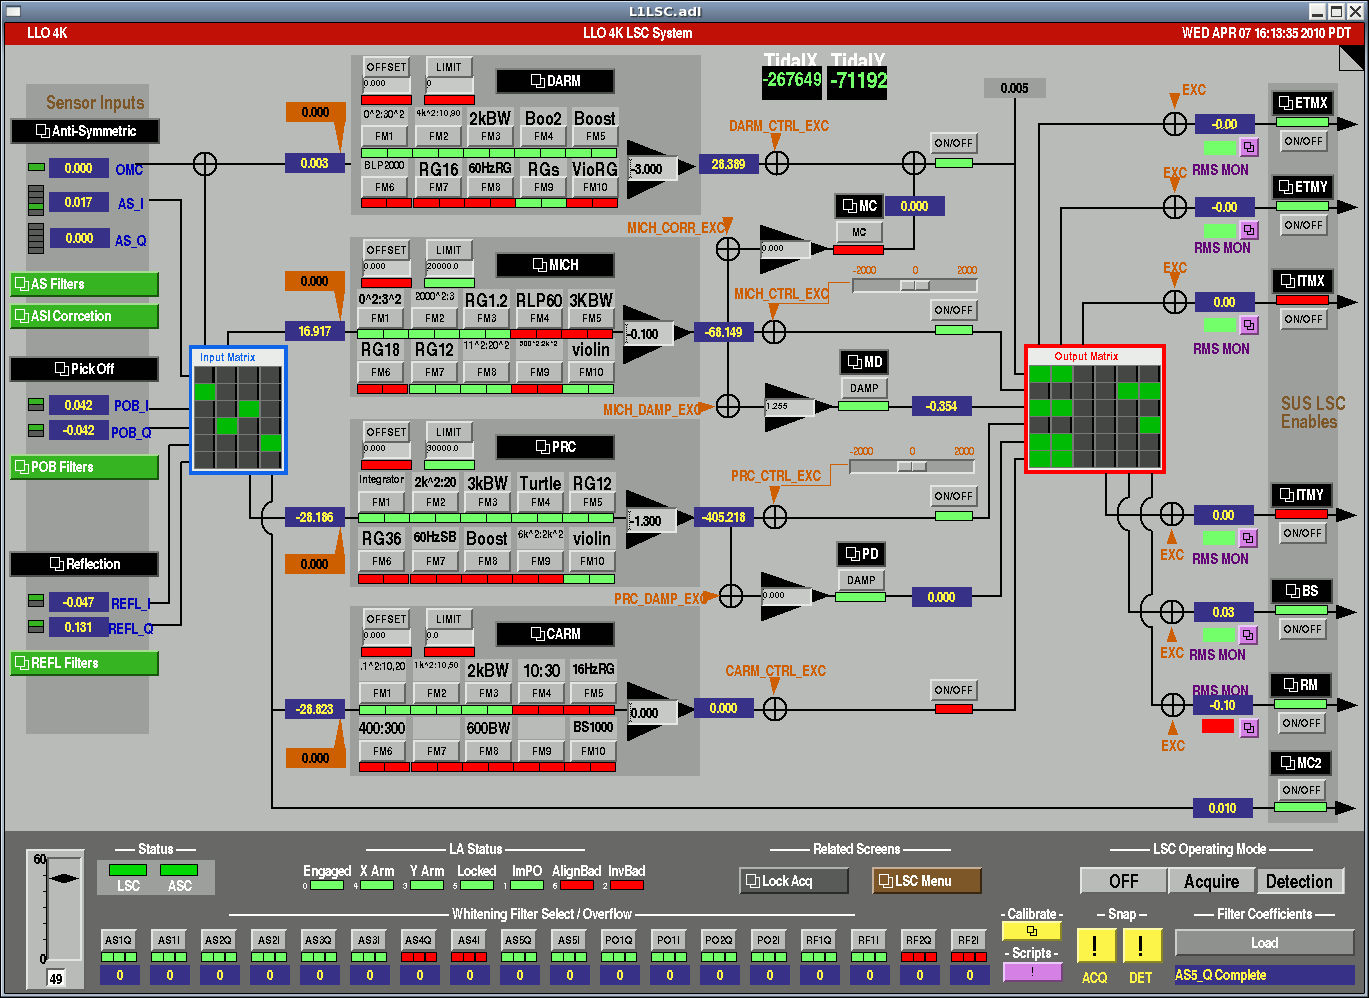
\includegraphics[width=\columnwidth]{figures/L1LSC.png}
\caption[Length Sensing and Control (LSC) control screen]{The control screen for the Length Sensing and Control
  subsystem at Livingston.  The control screen depicts signal flow in
  a generally left-to-right manner.  Photodiodes at the anti-symmetric
  (AS), pick-off (PO), and reflected (REFL) ports are indicated on the
  extreme left.  These signals are combined via an input matrix to
  form the DARM, MICH, PRC, and CARM degrees of freedom.  These
  signals are processed through an array of filter banks defining the
  control filters.  Finally, the signals pass through an output matrix
  and are then directed to the individual optics.}
\end{figure}

\section{Beam Diverter}

When the interferometer loses lock, the stored power must be dumped
somewhere. Typically, due to the presence of the power recycling mirror,
the stored power comes out the output port. This high-power transient
is sufficiently strong to burn the detection photodiodes. In order
to prevent this, one of the steering mirrors is used as a fast shutter.
It is able to zero the transmission through the OMC in approx 2 ms.

\begin{comment}
\section{Observed Beam Motion}

FIXME: Put in plots of the measured beam motion, for posterity.
\end{comment}

\section{The Front End}
\begin{comment}
% FIXME - Gaby says: This is very cute, but it may take too long to do
% a proper job... again, in the interest of time, you may just skip a
% description of the front end.

\begin{quote}
\emph{Be exhorted:} you really can predict the noise floor accurately--to
accept a noisy front end is one of the stupidest and most expensive
mistakes you can make in designing sensitive optical
instruments. Measure it, and make sure you can explain every half
decibel. -- Phil Hobbs, \emph{Building Electro-Optical Systems} \cite{Hobbs2009Building}
\end{quote}
\end{comment}

To achieve the touted SNR improvement of DC readout it is imperative
that the signal not be lost to optical losses, non-optimal photodiode
quantum efficiency, or electronics noise.

\subsection{Photodiodes}
% H1 OMC DC PDs
% https://dcc.ligo.org/DocDB/0005/T0900420/001/T0900420-v1.pdf

Sub-optimal photodiode efficiency counts as a loss just like any other
optical loss. 

The OMC photodiodes are configured in a reverse-biased,
photoconductive arrangement.  An ideal photodiode in such a
configuration will allow one charge carrier to cross the junction for
each incident photon.  The ratio of photocurrent to incident power on
the photodiode is its \emph{responsivity}.  The ratio of a
photodiode's actual responsivity to the ideal is its \emph{quantum
  efficiency}.  At 1064 nm the ideal responsivity is
%
\begin{equation}
\frac{q_e}{h \nu} = \frac{q_e \lambda}{h c} \approx 0.86 \text{ Amps/Watt}
\end{equation}
where $q_e\approx 1.6\times10^{-19}\text{ C}$ is the electron charge.

\begin{comment}
 h = 6.626068e-34;
 c = 299792458;
 lambda = 1064e-9;
 qe = 1.60217646e-19;
 responsivity = qe * lambda / (h * c)
\end{comment}

One lesson (re-)learned during Enhanced LIGO is the need to measure
the characteristics of every individual noise-sensitive component
installed in the final machine rather than relying on measurements of
test samples or typical values.  The photodiodes we originally
installed turned out to have quantum efficiency $\lesssim$ 0.60 while
the test articles of the same part number had quantum efficiency
within a few percent of unity.  Clearly there had been some change in
the manufacturing process that resulted in a greatly diminished
quantum efficiency.  Even for parts which do not show such a dramatic
systematic change, characteristics of individual parts come from some
distribution, and by measuring a batch of parts, the lowest noise
components can be hand picked.

In September 2009 we replaced the bad phototdiodes.  The replacement
photodiodes are Perkin Elmer 3mm InGaAs diodes, part number C30665GH.
The measured quantum efficiency was consistent with unity~\cite{Rollins2009H1}.

\subsection{Electronics}
An optical power of 100 mW on the readout photodiodes will produce a
photocurrent of $i = q_e\lambda/(hc)\cdot 100\text{ mW } = 86\text{ mA}$, which
in turn has a shot noise floor of $\sqrt{2 q_e i}\approx 500 \text{
  pA}/\sqrt{\text{Hz}}$.  Across $100\ \Omega$ transimpedance, this becomes $50
\text{ nV}/\sqrt{\text{Hz}}$.  The noise floor of the readout electronics must
be below this level and not be polluted by any baseband $1/f$ flicker noise.

The main strategy is to aggressively amplify the electronic signal as close to
the photodiodes as possible, so that noises added downstream become
insignificant.  To eliminate even triboelectric effects, the first preamp stages
are placed in-vacuum.  The in-vacuum preamps consist of active filter stages
with two zeros at 8 Hz and two poles at 80 Hz, for a factor of 100 amplification
at 100 Hz.  This is followed by two more pole-zero pairs in satellite amplifiers
on the floor outside the vacuum chamber, for a total gain of 10,000 before the
long run to the racks.

\begin{comment}
h = 6.626068e-34;
c = 299792458;
lambda = 1064e-9;
qe = 1.60217646e-19;
I = qe * lambda / (h * c)
sqrt(2* qe * I)
\end{comment}

%Additional references: \cite{Prijatelj2010,Bork2009ELIGO,Betzwieser2004Study}
